\documentclass{amsart}

\usepackage[english]{babel}
\usepackage[utf8]{inputenc}
\usepackage{graphicx}
\usepackage{mathtools}
\usepackage{amsthm}
\usepackage{thmtools,thm-restate}
\usepackage{amsfonts}
\usepackage{hyperref}
\usepackage[singlelinecheck=false]{caption}
\usepackage[backend=biber,url=true,doi=true,eprint=false,style=alphabetic]{biblatex}
\usepackage{enumitem}
\usepackage[justification=centering]{caption}
\usepackage{indentfirst}
\usepackage{algorithm}
\usepackage{algpseudocode}
\usepackage{listings}
\usepackage[x11names, rgb]{xcolor}
\usepackage{tikz}
\usepackage{hyperref}
\usepackage{subcaption}
\usepackage{booktabs}
\usepackage{linegoal}
\usepackage{csquotes}
\usetikzlibrary{snakes,arrows,shapes}

\addbibresource{references.bib}
\graphicspath{{imgs/}}

\makeatletter
\def\subsection{\@startsection{subsection}{3}%
  \z@{.5\linespacing\@plus.7\linespacing}{.1\linespacing}%
  {\normalfont}}
\makeatother

\makeatletter
\patchcmd{\@setauthors}{\MakeUppercase}{}{}{}
\makeatother

\DeclareMathOperator*{\argmin}{arg\,min}
\DeclareMathOperator*{\argmax}{arg\,max}
\DeclareMathOperator*{\Val}{\text{Val}}
\DeclareMathOperator*{\Ch}{\text{Ch}}
\DeclareMathOperator*{\Pa}{\text{Pa}}
\DeclareMathOperator*{\Sc}{\text{Sc}}
\newcommand{\ov}{\overline}

\newcommand\defeq{\mathrel{\overset{\makebox[0pt]{\mbox{\normalfont\tiny\sffamily def}}}{=}}}

\newcommand{\algorithmautorefname}{Algorithm}
\algrenewcommand\algorithmicrequire{\textbf{Input}}
\algrenewcommand\algorithmicensure{\textbf{Output}}
\algnewcommand{\LineComment}[1]{\State\,\(\triangleright\) #1}

\captionsetup[table]{labelsep=space}

\theoremstyle{plain}

\newcounter{dummy-def}\numberwithin{dummy-def}{section}
\newtheorem{definition}[dummy-def]{Definition}
\newcounter{dummy-thm}\numberwithin{dummy-thm}{section}
\newtheorem{theorem}[dummy-thm]{Theorem}
\newcounter{dummy-prop}\numberwithin{dummy-prop}{section}
\newtheorem{proposition}[dummy-prop]{Proposition}
\newcounter{dummy-corollary}\numberwithin{dummy-corollary}{section}
\newtheorem{corollary}[dummy-corollary]{Corollary}
\newcounter{dummy-lemma}\numberwithin{dummy-lemma}{section}
\newtheorem{lemma}[dummy-lemma]{Lemma}
\newcounter{dummy-ex}\numberwithin{dummy-ex}{section}
\newtheorem{exercise}[dummy-ex]{Exercise}
\newcounter{dummy-eg}\numberwithin{dummy-eg}{section}
\newtheorem{example}[dummy-eg]{Example}

\numberwithin{equation}{section}

\newcommand{\set}[1]{\mathbf{#1}}
\newcommand{\pr}{\mathbb{P}}
\newcommand{\eps}{\varepsilon}
\renewcommand{\implies}{\Rightarrow}

\newcommand{\bigo}{\mathcal{O}}

\setlength{\parskip}{1em}

\lstset{frameround=fttt,
	numbers=left,
	breaklines=true,
	keywordstyle=\bfseries,
	basicstyle=\ttfamily,
}

\newcommand{\code}[1]{\lstinline[mathescape=true]{#1}}
\newcommand{\mcode}[1]{\lstinline[mathescape]!#1!}


\title{%
  \noindent\rule{13cm}{1.0pt}\\
  \vspace{0.2cm}
  The Poon-Domingos Parameter Learning Algorithm for Image Completion and Classification on
  Sum-Product Networks
  \noindent\rule{13cm}{0.8pt}
}
\xdef\shorttitle{The Poon-Domingos Algorithm}
\author[]{\normalsize\textbf{Renato Lui Geh}\\\small Computer Science\\Institute of Mathematics
  and Statistics\\University of São Paulo\\\texttt{renatolg@ime.usp.br}}

\begin{document}

\begin{abstract}
  In this document we describe the Poon-Domingos~\cite{poon-domingos} parameter learning algorithm
  for image classification and completion.
  \vspace*{-3.5em}
\end{abstract}

\maketitle

\section{Structure}

The Poon-Domingos algorithm uses a fixed structure and then learns the weights through generative
learning. We first give an overview on how to build the structure given an image and then provide a
pseudo-code algorithm for building such structure.

\subsection{Overview}

The Poon architecture models a probability distribution over a set of images. It is constructed by
taking all possible rectangular axis-aligned regions in the image and assigning product nodes to
each of these regions. Two sum nodes are then added as children for each of these regions,
representing all the possible pairings of subregions in each region determined by the axis-aligned
division set in the previous step. We then add the product nodes to a single sum node that
represents the undivided original area. We then recursively apply the same steps on each sum node
we constructed this way, taking that sum node as the new root of the sub-SPN\@. The Poon structure
accepts different multiple resolution levels. At every region splitting, we consider a step $r$
that indicates how fine the granularity is for the architecture.

\begin{figure}[h]
  \centering
  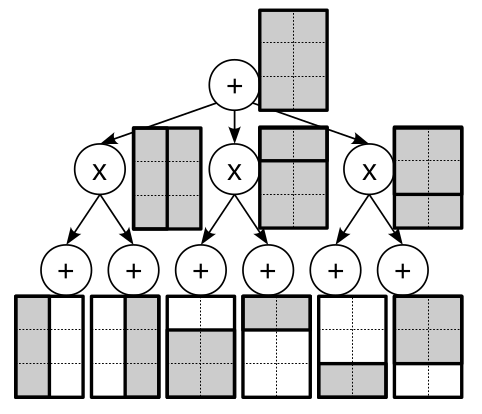
\includegraphics[scale=1.0]{dv_spn.png}
  \captionsetup{justification=raggedright}
  \caption{The Poon architecture with $r = 1$ resolution. At each product node division, we
  consider an $r$ length division on each axis. Since $r=1$ in this case, we have $3$ product
  nodes, with each of their two possible subregions represented by sum nodes. Note how product
  nodes are always decomposable and sum nodes are always complete.\label{fig:dv_spn}}
\end{figure}

\subsection{Definitions and properties}

Let us organize in a clearer way what we have extracted from~\cite{clustering}.

\begin{definition}[Region] A region $\pi$ is a product node. Graphically, it represents an
  axis-aligned rectangular region of the image. We shall denote an SPN $S(\cdot)$ rooted at a
  region as $\pi(\cdot)$.
\end{definition}

\begin{definition}[Subregion] A subregion $\sigma$ is a sum node. Given a region $R$, the children
  of $R$ are the two possible rectangles that compose $R$. We shall denote an SPN rooted at a
  subregion as $\sigma(\cdot)$.
\end{definition}

The idea behind the Poon structure algorithm is to recursively take a rectangular subarea of an
image and divide it into all $k$ possible regions given a granularity $r$, with each region having
two children (subregions) that represent the possible pairings of each region. We then recurse
through each of these subregions.

Let $I (x_0, y_0, x_1, y_1)$ be the area of the image we are to create the structure for, with
$ (x_0, y_0)$ and $ (x_1, y_1)$ being the top left and bottom right positions in the image. The
entire image is given by $I (0, 0, w, h)$, where $w, h$ are the width and height of the image
respectively.

A subregion $\sigma$ implicitly represents an area $I (x_0, y_0, x_1, y_1)$, whilst each region of
$\sigma$ is a possible subdivision of $I$ by drawing a line, either horizontally or vertically,
through one of the axis of $I$, partitioning it into two subregions.

We can clearly see that, for a subregion $\sigma$, there are $x_1-x_0$ possible vertically divided
regions and $y_1-y_0$ horizontally divided regions, bringing the total to $ (x_1+y_1)- (x_0+y_0)$
possible product nodes as children of $\sigma$ for $r=1$. For the general case, we can clearly see
that we have $\lceil (x_1-x_0)/r\rceil + \lceil (y_1-y_0)/r\rceil$ possible regions.

%\begin{proposition} The height of a Poon-Domingos SPN structure is $2w+2h-3$.
%\end{proposition}
%\begin{proof}
  %Let $h$ be the height of an SPN $S$. Maximizing $h$ is finding the longest path $p$ from a leaf
  %(in this case the image's pixel) to the root node. Let us assume $(x, y)$ as the farthest leaf's
  %pixel representation from the root node. Since a region cuts an area $I$ either horizontally or
  %vertically, with each subregion being the two possible subregions, we can easily see that in
  %order to maximize $p$ we must maximize the number
%\end{proof}

\subsection{Algorithm}

The structure algorithm is recursive. It takes as parameters a sum node $S$ as root of the SPN, the
$ (x_0,y_0)$ top-left position of the subregion $S$ relative to the original complete image, the
$ (x_1,y_1)$ bottom-right position of the subregion $S$, the resolution granularity step $k$ and a
dataset $\mathcal{D}$ where $\mathcal{D}[X]$ is the set of instances of variable $X$.

\begin{algorithm}[H]
  \caption{\code{GenerateDenseSPN}}\label{alg:structure}
  \begin{algorithmic}[1]
    \Require\,Root sum node $S$
    \Require\,Top-left position $p_0= (x_0,y_0)$ of the underlying image area of $S$
    \Require\,Bottom-right position $p_1= (x_1,y_1)$ of the underlying image area of $S$
    \Ensure\,A dense SPN structure
  \end{algorithmic}
\end{algorithm}


%--------------------------------------------------------------------------------------------------

\printbibliography[]

\end{document}
